\documentclass[12pt]{article}
\usepackage{graphicx}
\usepackage{xcolor}
\usepackage{colortbl}
\usepackage{tikz}
\usepackage{amsmath}
\usepackage{caption}
\usepackage{subcaption}
\usepackage{textcomp}
\usepackage{tabulary}
\usepackage{float}
\usepackage{hyperref}

\begin{document}
\begin{titlepage}
\begin{center}
    
\includegraphics[width=\textwidth]{./logo.png}
    \\ [2.5cm]
    \textsc{\Large Autonomous Mobile Robots}
    \\ [0.5cm]
    \textsc{\large Third assignment}
    \\ [1cm]
    \hrule
    \vspace{0.3cm}
    \textsc{Probabilistic Pose Estimation based on a Topological Map}
    \\ [0.3cm]
    \hrule
    \vfill
    \textsc{Ruben Janssen, 10252657 \\[0.7cm] Department of Computer Science \\ University of Amsterdam \\[0.3cm] \today}
\end{center}
\end{titlepage}
\tableofcontents
\clearpage
\section{Introduction}
In order for an autonomous mobile robot to drive and navigate, it requires some method by which to determine its position. This is called the localization problem. One of the methods to solve this problem is by using probabilistic pose estimation based on a topological map. The robot tries to estimate its position with respect to known locations in the environment. This can be achieved by comparing its current position to known locations and estimating which locations is most similar. The most similar location is most probably the current location of the robot.

\section{Setup}
The robot used for the experiment is a lego NXT-Robot. A camera is attached on top of this robot. In front of this camera a mirror is placed to provide an omnidirectional view. 

\subsection{Dataset}
To compare the current position of the robot with known locations, a dataset of known locations is needed. Due unavailability of robots, a dataset of pictures is used to compare the locations with, rather than comparing the known locations to a live input feed.
An experiment environment was set up to test the robot. This environment simulated walls with tape, to allow the robot to detect the 'walls'. An important feature of this environment is that it is closed and finite.
For the dataset, 8 pictures were taken that are distributed over the whole environment as shown in the figure. Another 8 have been taken distributed over the environment to experiment with.

\begin{figure}[H]
	\centering
	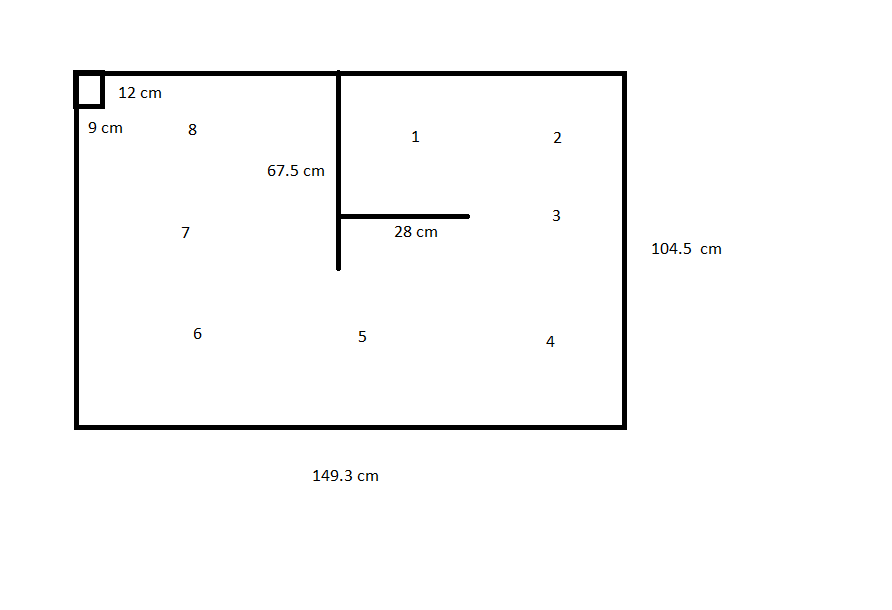
\includegraphics[width=\textwidth]{Opzet.png}
	\caption{Map of known locations}
\end{figure}

\subsection{Parameters}
In order to analyse the pictures, some parameters had to be set. As all pictures were made with the same camera, the center coordinates of the are set to (545,400). Also, the degree of curvature of the mirror $\alpha$ is set to 140. The height of the camera is set to 21 cm. These values are all needed to determine the distances between the robot and the wall. The Rmin and Rmax values are set to 115 and 170 respectively. These determine the distances in pixels the robot analyses. Pixels closer than 115 are ignored as the often consist of images of the robot itself. Pixels farther than 170 are often not important, as seen in the figure below.

\begin{figure}[H]
	\centering
	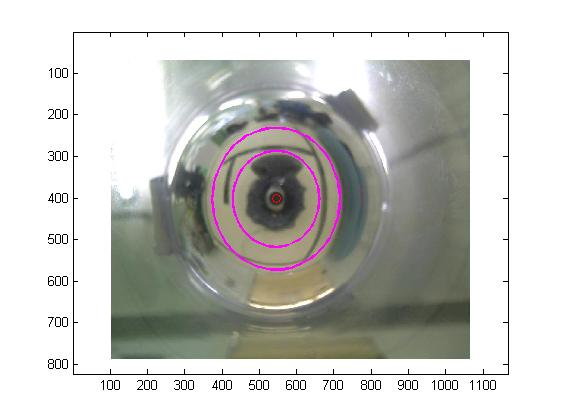
\includegraphics[width=\textwidth]{radius.jpg}
	\caption{Range of Rmin and Rmax the robot uses to detect}
\end{figure}

\section{Implementation}
\subsection{Detecting Line Fingerprints}
Before pictures can be compared to localize the robot, they have to be analysed. First, the walls are detected around the robot (4). Second, the detected walls are mapped on a grid corresponding with their distance from the vehicle (5). Third, the lines are extracted from the grid (6).

\begin{figure}[H]
	\centering
	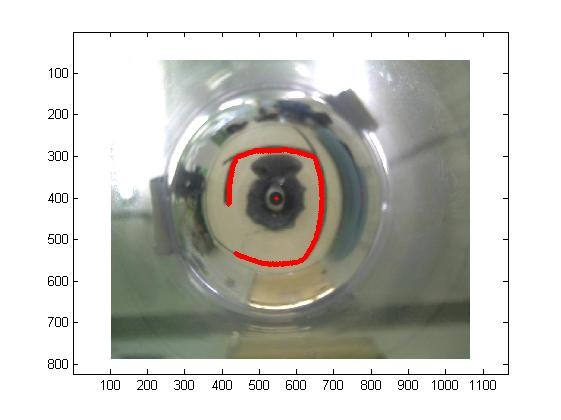
\includegraphics[width=0.8\textwidth]{points.jpg}
	\caption{Range of Rmin and Rmax the robot uses to detect}
\end{figure}

\begin{figure}[H]
	\centering
	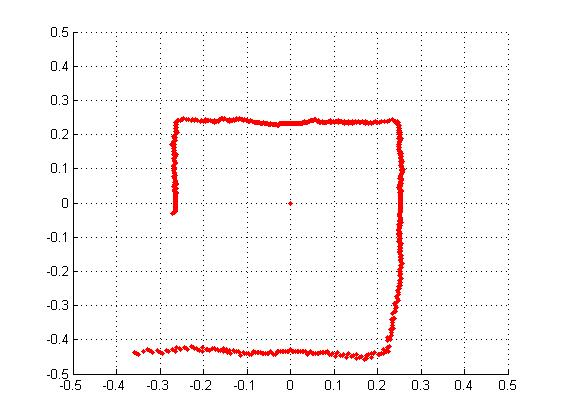
\includegraphics[width=0.8\textwidth]{grid.jpg}
	\caption{Range of Rmin and Rmax the robot uses to detect}
\end{figure}

\begin{figure}[H]
	\centering
	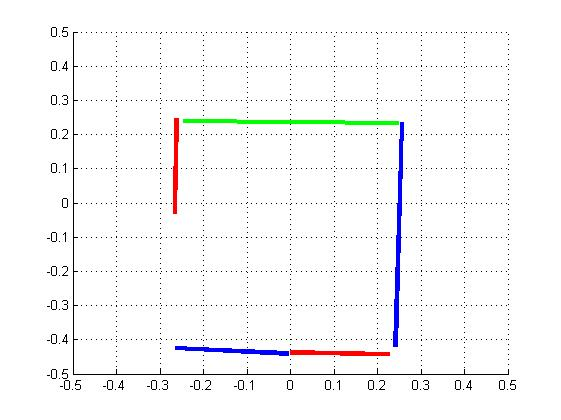
\includegraphics[width=0.8\textwidth]{lines.jpg}
	\caption{Range of Rmin and Rmax the robot uses to detect}
\end{figure}

The code to determine points and calculate the distance grid are provided. Same goes for the code to extract the lines. To extract the lines from the distance grid, a simplified version of the Split \& Merge algorithm is used. In order for the Split \& merge algorithm to work well, a lot of detection points are required. Small errors or noise can easily disturb the algorithm. In figure 3 for example, the line at the bottom is split in two parts. Also, the line stops earlier than it should. The lines are wrongly determined due small errors. These wrong lines might result into wrong position estimations, as these estimations are based on the lines.

\subsection{Comparing Line Based Fingerprints}
Once all pictures are analysed, the line fingerprints can be compared. Comparing is done by calculating the Levenshtein distance\\ (\url{www.en.wikipedia.org/wiki/Levenshtein_distance}) between the two pattern strings that represent the line fingerprints of the images. However, as the robot is based on probability estimations, the Levenshtein distance is not enough. In order to calculate the probability of a robot to be somewhere, the following formula is used:\\\\
$SimilarityProb = \dfrac{StringLength - LevenshteinDistance}{StringLength} \times 100\%$\\\\
Based on the string length and the Levenshtein distance, the probability of the location of the robot is determined. If the Levenshtein distance is 0, the robot must be exactly at the same position as the known location. However, if the Levenshtein distance is large, the robot has a very different than the known location and the probability of being at the same location is small.

As the dataset consists of 8 known locations and 8 random positions, a probability matrix can be made as shown in the following figure:

\begin{figure}[H]
	\centering
	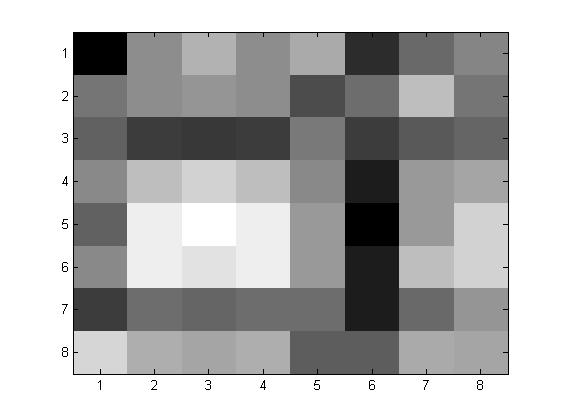
\includegraphics[width=\textwidth]{lines_chance.jpg}
	\caption{Probability matrix of line segments. A lighter color represents a higher chance. On the X-axis of the figure, the known locations are represented from 1 to 8. On the Y-axis, the test locations are represented.}
\end{figure}

\subsection{Detecting Blob Based Fingerprints}
Another method to determine fingerprints of an image is by using blobs. Provided code extracting colored blobs by using color thresholds. However, as the testing environment has no colors, the blobs are based only on black and white values. To determine the blobs, each pixel is analysed and if it passes the black threshold, it is considered to be part of a blob. 

\begin{figure}[H]
	\centering
	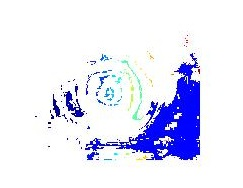
\includegraphics[width=0.6\textwidth]{blobs.jpg}
	\caption{Detected blobs}
\end{figure}

\subsection{Comparing Blob Based Fingerprints}
Blobs can also be represented as a pattern string. To determine this string, not the all blobs are used. However, only the blobs within the Rmin and Rmax rang are considered. Based on this pattern string, the same method is used as to compare line fingerprints to calculate the probability.

\begin{figure}[H]
	\centering
	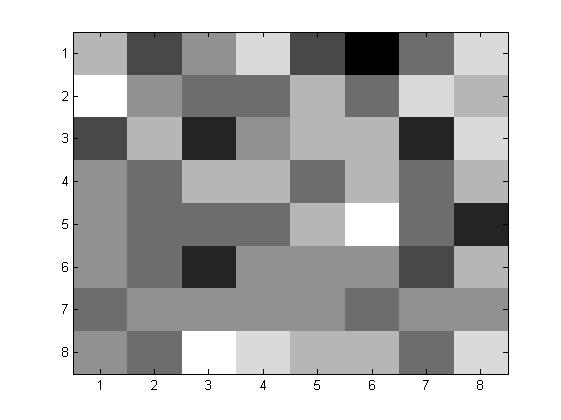
\includegraphics[width=\textwidth]{blobs_chance.jpg}
	\caption{Detected blobs. On the X-axis of the figure, the known locations are represented from 1 to 8. On the Y-axis, the test locations are represented.}
\end{figure}

\subsection{Combining Blob Based and Line Based Fingerprints}
As line based and blob based fingerprints are prone to errors, a combination can be used to determine more accurate probabilities. However, there are two ways to combine the different types of fingerprints.
\subsubsection{Weighted Average}
The simplest way of combining the two types of fingerprints is by using a weighted average. In this method, the probabilities are calculated by both types and the average of both probabilities is the final probability. However, by weighting one of the types, a better balance can be achieved if one of the two is a better estimator. After experimenting, the best results were achieved by setting the weight of line based fingerprints to 0.33 and setting the blob based fingerprints to 0.66. This resulting in the following probability matrix:

\begin{figure}[H]
	\centering
	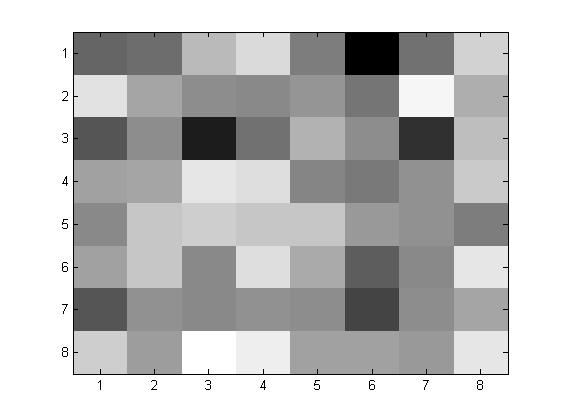
\includegraphics[width=\textwidth]{lines_and_blobs_chance_weighted.jpg}
	\caption{Probability based on the weighted average of blob and line patterns. On the X-axis of the figure, the known locations are represented from 1 to 8. On the Y-axis, the test locations are represented.}
\end{figure}

\subsubsection{Pattern Concatenation}
Another method to combine the two types of fingerprints is by concatenation of the pattern strings. By concatenating the blob and line pattern string, the Levenshtein distance can be calculated based on both fingerprints. This results in the following probability matrix:

\begin{figure}[H]
	\centering
	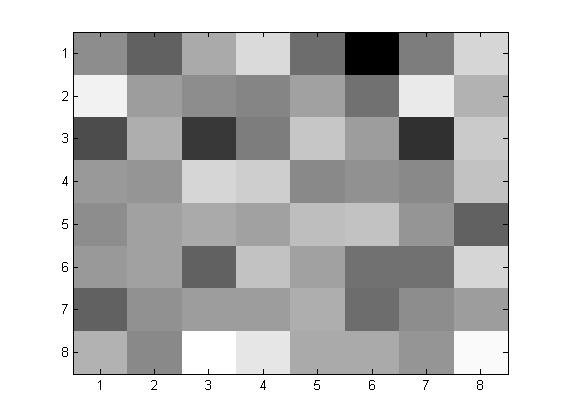
\includegraphics[width=\textwidth]{lines_and_blobs_chance_fusion.jpg}
	\caption{Probability based on the concatenation of blob and line patterns. On the X-axis of the figure, the known locations are represented from 1 to 8. On the Y-axis, the test locations are represented.}
\end{figure}

\section{Results}
In the following two tables the results of the experiments are compared with the real locations:

\begin{table}[H]
  \centering
  \begin{tabulary}{\textwidth}{| C | C | C | C |}
    \hline
    Experiment & Corresponding Known Location & Line Fingerprint Estimated Location & Blob Fingerprint Estimated Location \\ \hline
    1 & 7 or 8 &  3 or 5 & 4 or 8\\ \hline
    2 & 7 or 8 &  7 & 1\\ \hline
    3 & 4 or 5 &  1 or 6 & 5 or 6 or 8\\ \hline
    4 & 2 &  2 or 3 or 4 & 2 or 3 or 6\\ \hline
    5 & 8 &  2 or 3 or 4 & 6\\ \hline
    6 & 8 &  2 or 3 or 8 & 8\\ \hline
    7 & 6 or 7 & 8 & 7 or 8\\ \hline
    8 & 1 or 2 & 1 & 3\\ \hline
  \end{tabulary}
  \caption{Results Line and Blob Fingerprints}
  \label{tab:linelength}
\end{table}

\begin{table}[H]
  \centering
  \begin{tabulary}{\textwidth}{| C | C | C | C |}
    \hline
    Experiment & Corresponding Known Location & Weighted Average Estimated Location & Pattern Concatenation Estimated Location \\ \hline
    1 & 7 or 8 & 4 or 8 & 4 or 8\\ \hline
    2 & 7 or 8 & 7  & 1 or 7\\ \hline
    3 & 4 or 5 & 5 or 8 & 5 or 8\\ \hline
    4 & 2 & 3 or 4 & 3 or 4\\ \hline
    5 & 8 & 3 & 5 or 6\\ \hline
    6 & 8 & 4 or 8 & 4 or 8\\ \hline
    7 & 6 or 7 & 2 or 5 or 8 & 5\\ \hline
    8 & 1 or 2 & 3 or 4 & 3 or 8\\ \hline
  \end{tabulary}
  \caption{Results Weighted Average and Pattern Concatenation}
  \label{tab:linelength}
\end{table}

As can be deducted from the tables, the algorithms do not work as optimal as they should. This is mainly caused because the algorithms are not rotation invariant. Unfortunately, the provided dataset is not consisted in orientation. As the rotation of the robot differs, the lines and blobs do not match. A rotation invariant algorithm would provide much more accurate results. This could be achieved by using sift or RANSAC.

An interesting result is the difference between the weighted average and the pattern concatenation algorithms. While the two separate methods differ greatly in the predictions they make, the algorithms that combine the two methods are very similar. This indicates that the algorithms work similarly well.

\section{Conclusion}
In conclusion, the algorithms seem to be greatly disturbed by the difference in orientation of the robot. However, even while the algorithms are not rotation invariant, all algorithms have an accuracy of 40\% to 50\%. A rotation invariant algorithm would greatly increase the accuracy.
\end {document}